\documentclass[11pt]{beamer}

\graphicspath{{assets/}{../}{./}}

\usepackage{booktabs}
\usepackage{multicol}
\usepackage{tikz}
\usetikzlibrary{positioning}
\usepackage[utf8]{inputenc}
\usepackage[T1]{fontenc} 
\usepackage{amsmath}
\usepackage{graphicx}
\usepackage[english]{babel}

\usetheme{Madrid}

% -------- FOOTER PERSONALIZADO --------
\newcommand{\eventname}{Bayesian Inference}

\setbeamertemplate{footline}{
  
  \leavevmode%
  \hbox{%
    \begin{beamercolorbox}[wd=.33\paperwidth,ht=2.7ex,dp=1.2ex,leftskip=0.8em]{author in head/foot}%
      \usebeamerfont{author in head/foot}\insertshortauthor
    \end{beamercolorbox}%
    
    \begin{beamercolorbox}[wd=.34\paperwidth,ht=2.7ex,dp=1.2ex,center]{title in head/foot}%
      \usebeamerfont{title in head/foot}\eventname
    \end{beamercolorbox}%
    
    \begin{beamercolorbox}[wd=.33\paperwidth,ht=2.7ex,dp=1.2ex]{date in head/foot}%
      \hfill
      \usebeamerfont{date in head/foot}
      \ifx\insertsection\empty
        \eventname
      \else
        \insertsection
      \fi
      \hspace{0.5em} | \hspace{0.5em}
      \insertframenumber/\inserttotalframenumber
      \hspace{0.8em}
    \end{beamercolorbox}%
  }%
  \vskip0pt%
}

\usefonttheme{default}
\usepackage{palatino}
\usepackage[default]{opensans}
\useinnertheme{circles}

% --- UPRM Green ---
\usepackage{xcolor}
\definecolor{uprmgreen}{RGB}{0,102,51}
\setbeamercolor{structure}{fg=uprmgreen}

% Avoid hyperref warnings
\pdfstringdefDisableCommands{%
  \def\\{}%
  \def\and{, }%
}

%------------------------------------------------
% TITLE INFORMATION
%------------------------------------------------

\title{Estimation of Change in \\ Population of municipalities in PR}

\author[Ouslan]{\small{
Alejandro M. Ouslan \& Tatiana E. Crespo}}

\institute[UPRM]{University of Puerto Rico, Mayagüez}
\titlegraphic{
\includegraphics[width=2cm]{UPR.png}}

\date[\today]{\small{[ESMA 6835]: Inferencia Bayesian}\\
\vspace{2mm}
\footnotesize{\today}}

%------------------------------------------------
% CUSTOM TITLE PAGE
%------------------------------------------------

\setbeamertemplate{title page}{
  \vbox{}
  \vfill
  \begin{center}

    \begin{beamercolorbox}[sep=12pt,center,rounded=true,shadow=true]{title}
      {\usebeamerfont{title}\inserttitle\par}
    \end{beamercolorbox}

    \vspace{0.4cm}

    {\usebeamerfont{author}\insertauthor\par}

    \vspace{0.3cm}

    \inserttitlegraphic

    \vspace{0.3cm}

    {\usebeamerfont{date}\insertdate\par}

  \end{center}
  \vfill
}

%------------------------------------------------
\begin{document}

{
\setbeamertemplate{footline}{}
\setbeamertemplate{headline}{}
\begin{frame}
	\titlepage
\end{frame}
}

%------------------------------------------------
% TABLE OF CONTENTS
%------------------------------------------------

\section*{Presentation Overview}
\begin{frame}{Presentation Overview}

	\begin{columns}[T,onlytextwidth]
		\column{0.5\textwidth}
		\tableofcontents[sections={1-3}]

		\column{0.5\textwidth}
		\tableofcontents[sections={4-6}]
	\end{columns}

\end{frame}

\section{Introduction}
%------------------------------------------------

\begin{frame}{Introduction}

	\begin{itemize}
		\item Demographic change is an important topic for governments and policymakers.
		\item Understanding population characteristics is particularly important for regional governments.
		\item Anticipating population change helps guide infrastructure and public investment decisions.
	\end{itemize}

\end{frame}

%------------------------------------------------
\section{Methodology}
%------------------------------------------------

\begin{frame}{Methodology}

	\begin{itemize}
		\item Data obtained from the American Community Survey (ACS) 5-year estimates U.S. Census Bureau
		\item Population estimates from 2011 to 2023 were used.
		\item Dataset includes all 78 municipalities in Puerto Rico.
	\end{itemize}

\end{frame}

\begin{frame}{Methodology}
	The variables to consider for our simple regression model are:
	\begin{itemize}
		\item \textbf{Independent variable $X$:} the years for which we have population estimates for Puerto Rico
		\item \textbf{Dependent variable $Y$:} the total population for the 78 municipalities of Puerto Rico for each year
	\end{itemize}

\end{frame}

\begin{frame}{Methodology}

	The simple linear regression model to be used is the following:

	\[
		Y_i = \beta_0 + \beta_1 X_i + \epsilon_i
	\]

	where:
	\begin{itemize}
		\item $Y_i = $ population in year $i$
		\item $X_i = $ year
		\item $\beta_0 = $ intercept
		\item $\beta_1 = $ population change rate
		\item $\epsilon_i = $ random error
	\end{itemize}


\end{frame}

%------------------------------------------------
\section{Results}
%------------------------------------------------

\begin{frame}{Results}
	\begin{itemize}
		\item A \textbf{classical linear regression} was performed with a significance level of $\alpha = 0.05$, from which we obtained a population change rate of $-210.52$, indicating that the total population decreases each year.
		\item However, upon reviewing the p-value of this test (0.540), we realized that our findings are not statistically significant.
		\item Therefore, based on classical inference, there is insufficient evidence to determine that there is a drastic change in the population decrease over time in this model.
	\end{itemize}
\end{frame}

\begin{frame}{OLS Regression Results}
	\centering

	\textbf{Model Summary}

	\begin{tabular}{lc}
		\hline
		Observations       & 1014   \\
		R-squared          & 0.000  \\
		Adj. R-squared     & -0.001 \\
		F-statistic        & 0.3759 \\
		Prob (F-statistic) & 0.540  \\
		Durbin-Watson      & 1.935  \\
		\hline
	\end{tabular}

	\vspace{0.5cm}

	\textbf{Coefficients}

	\begin{tabular}{lcccc}
		\hline
		Variable  & Coef               & Std. Err           & t      & p-value \\
		\hline
		Intercept & $4.61\times10^{5}$ & $6.93\times10^{5}$ & 0.666  & 0.506   \\
		year      & -210.52            & 343.34             & -0.613 & 0.540   \\
		\hline
	\end{tabular}

\end{frame}


\begin{frame}{Results}
	\begin{itemize}
		\item Regarding the \textbf{Bayesian regression}, we obtained that the mean of the posterior distribution of the coefficient corresponding to the years is $-211.04$. This indicates that the population decreases per year.
		\item Furthermore, reviewing the Bayesian confidence intervals, it was found that there is a 94\% probability that the year effect is between -822.54 and 444.45. Thus, not statistically significative.
	\end{itemize}

\end{frame}


\begin{frame}{Bayesian Regression Results}
	\centering

	\begin{tabular}{lccc}
		\hline
		Parameter & Mean      & SD        & 94\% HDI                 \\
		\hline
		Intercept & 462101.05 & 690822.24 & [-866169.01, 1689104.77] \\
		year      & -211.04   & 342.49    & [-822.54, 444.45]        \\
		$\sigma$  & 40949.25  & 931.07    & [39207.54, 42669.78]     \\
		\hline
	\end{tabular}

	\vspace{0.4cm}

	\footnotesize
	Effective sample size ($ESS_{bulk}$) $\approx$ 5354--6805, $\hat{R}=1.00$ (good convergence).

\end{frame}


\begin{frame}{Results}
	\begin{itemize}
		\item Regarding the MCMC chains, the chains appear to blend quite well, and the R-squared value is approximately 1, suggesting that the model converged correctly.

	\end{itemize}

\end{frame}

%------------------------------------------------
\subsection{Densities}
%------------------------------------------------

\begin{frame}{Densities}

	\begin{figure}[H]
		\centering
		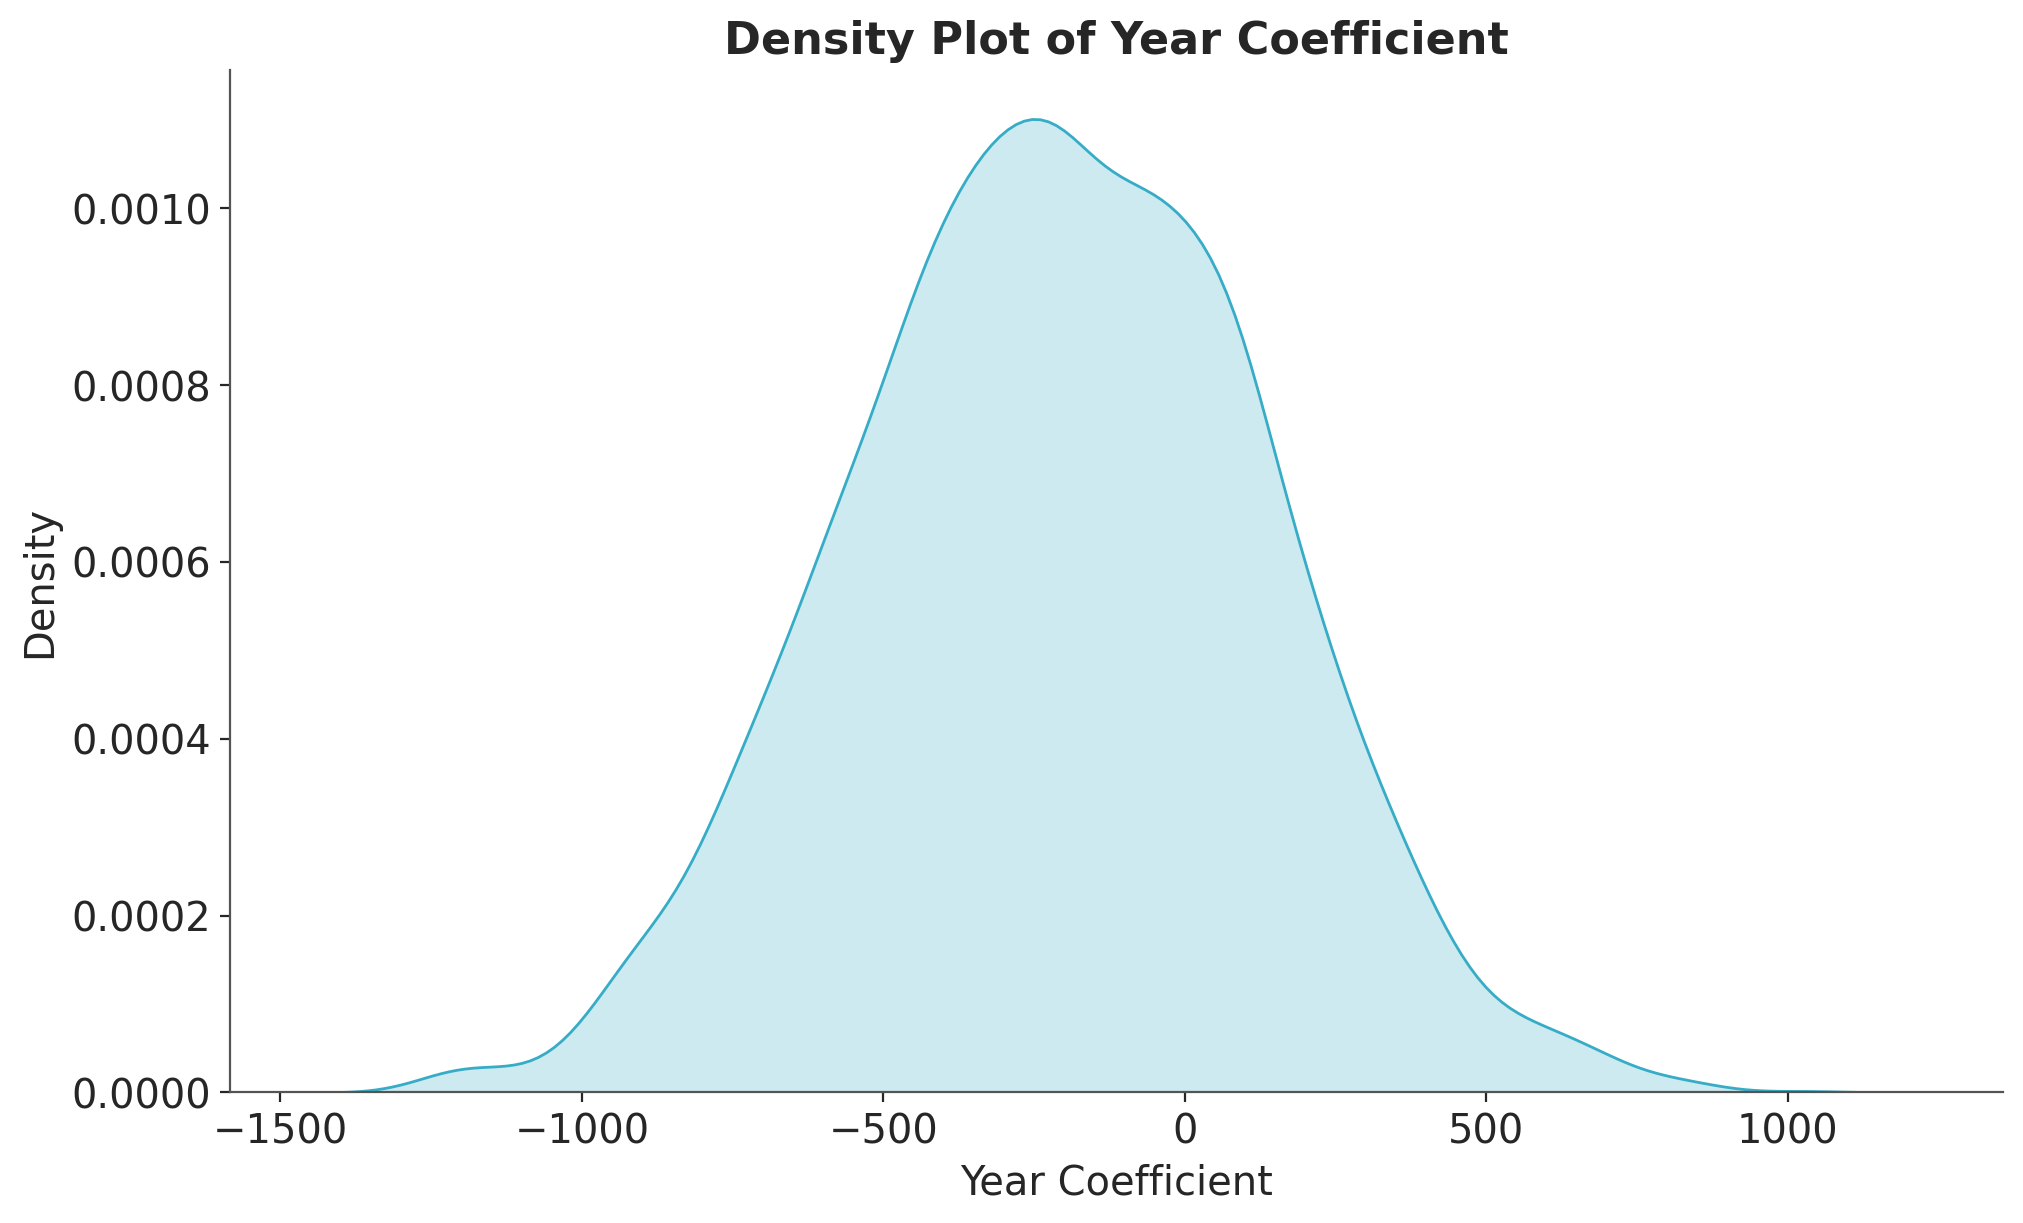
\includegraphics[width=0.4\textwidth]{assets/density.png}
	\end{figure}
\end{frame}

%------------------------------------------------
\subsection{Confidance Interval}
%------------------------------------------------

\begin{frame}{Confidance interval}
	\begin{figure}[H]
		\centering
		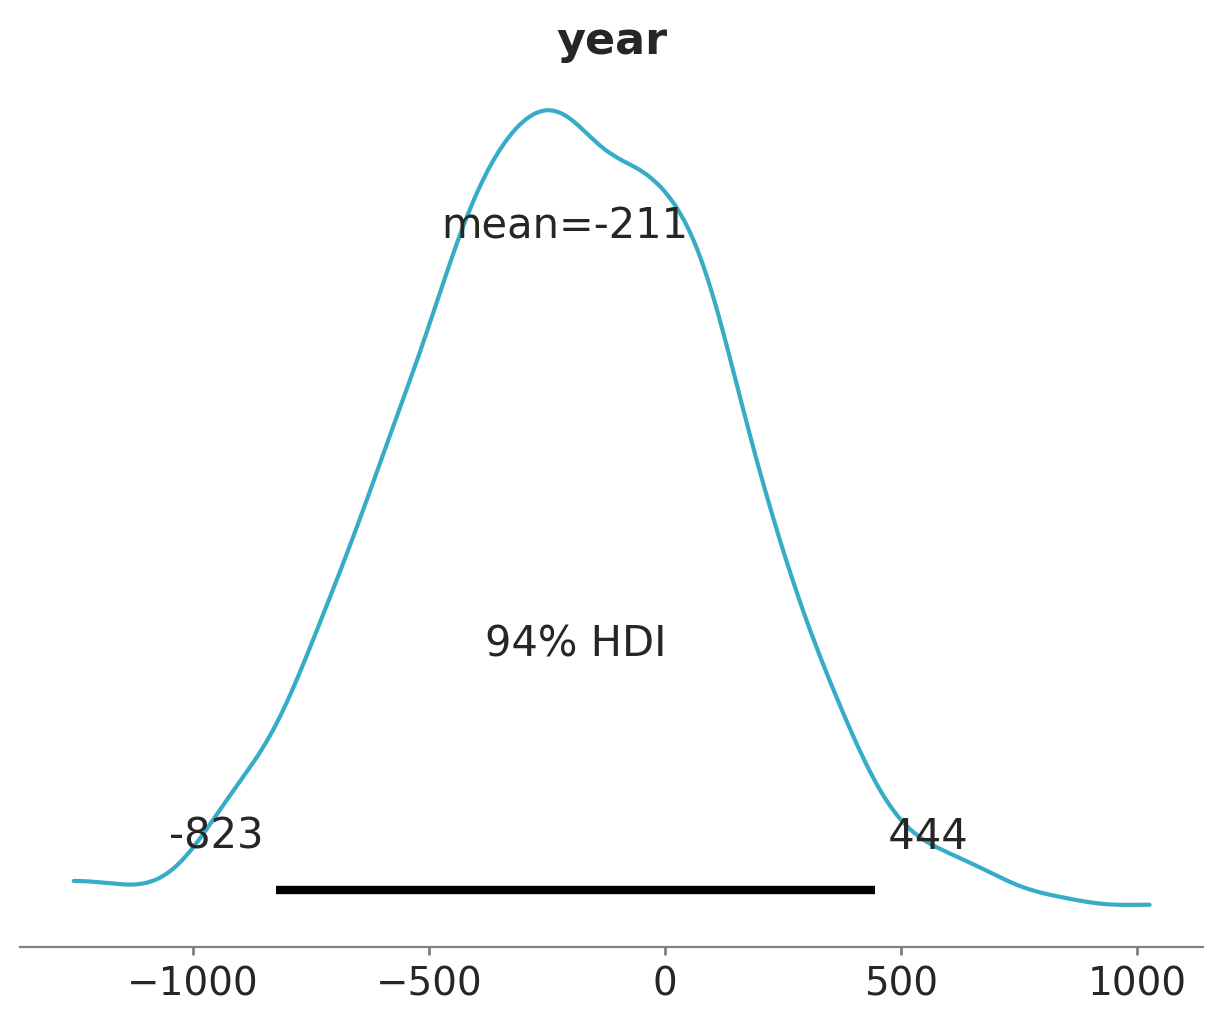
\includegraphics[width=0.4\textwidth]{assets/confidence.png}
	\end{figure}
\end{frame}
%------------------------------------------------
\subsection{Credibility Interval}
%------------------------------------------------

\begin{frame}{Credibility Interval}
	\begin{figure}[H]
		\centering
		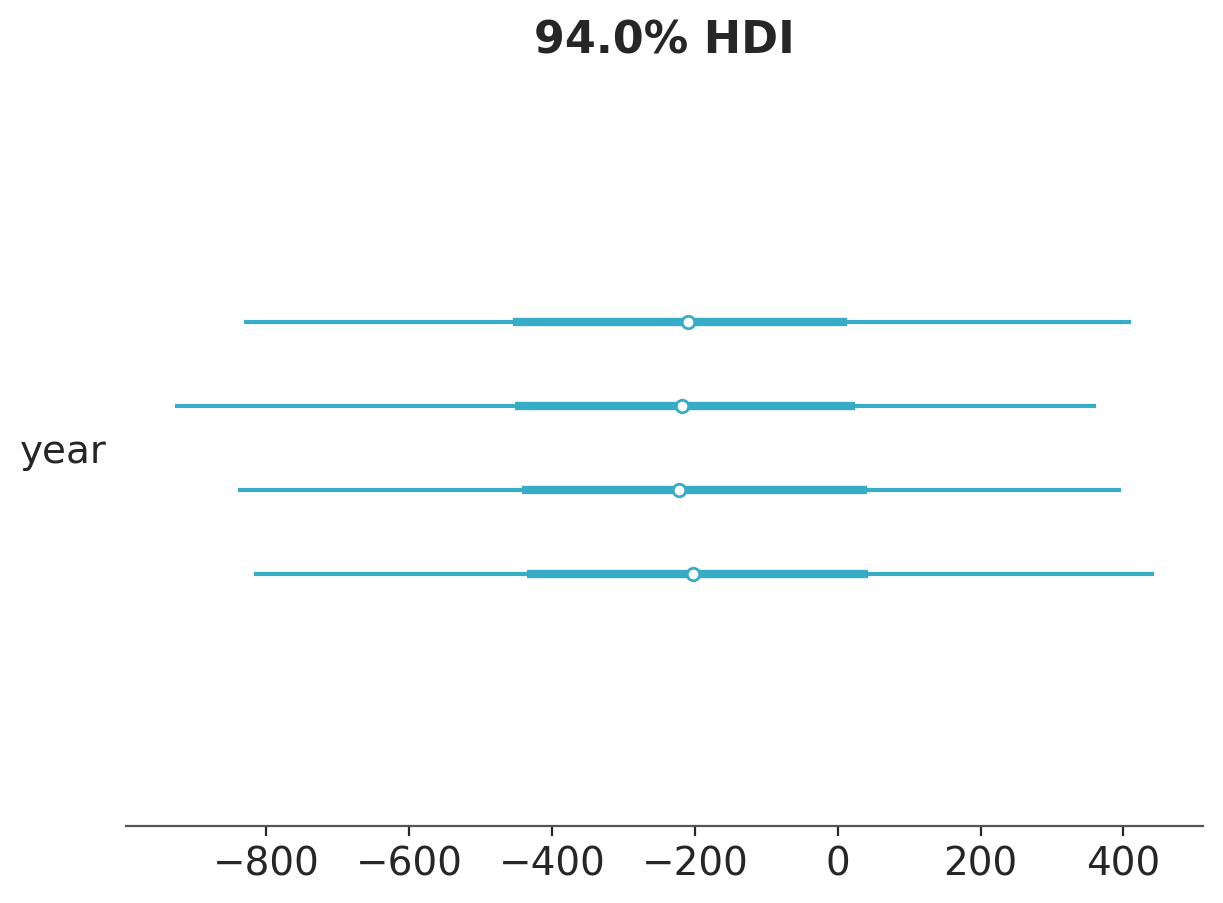
\includegraphics[width=0.4\textwidth]{assets/credibility intervals.png}
	\end{figure}
\end{frame}

%------------------------------------------------
\subsection{Distribution}
%------------------------------------------------

\begin{frame}{Distribution}
	\begin{figure}[H]
		\centering
		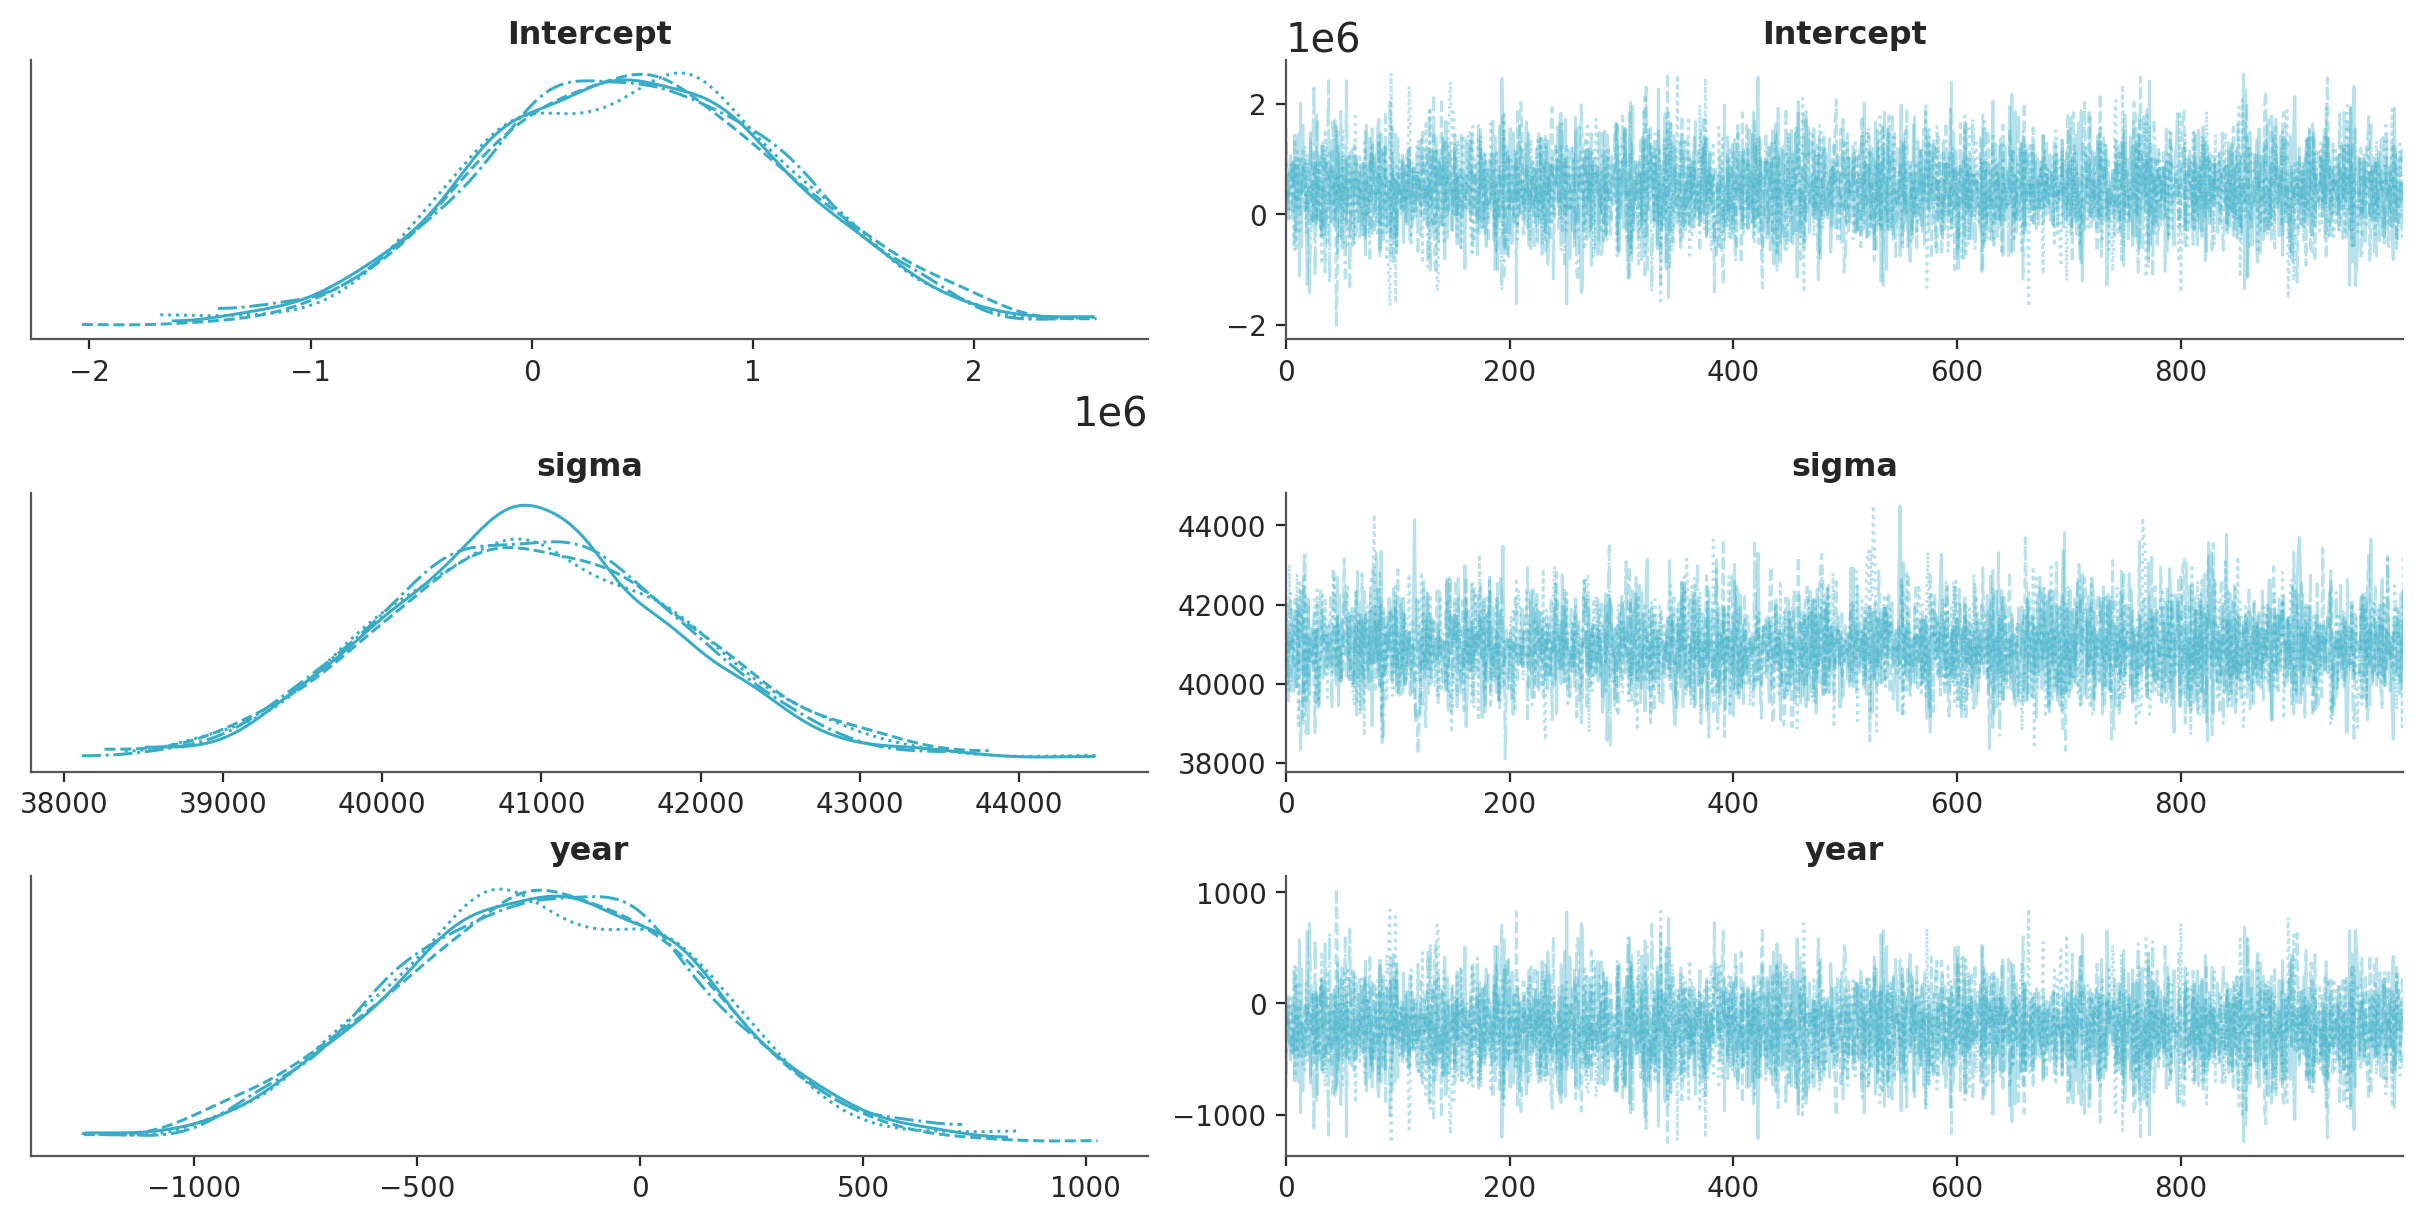
\includegraphics[width=0.4\textwidth]{assets/trace.png}
	\end{figure}
\end{frame}


%------------------------------------------------
\section{Predictions}
%------------------------------------------------

\begin{frame}{Predictions}

	\begin{itemize}
		\item Results did not show statistically significant changes over time.
		\item Due to this lack of significance, strong predictive conclusions cannot be made.
		\item No meaningful recommendations can be derived from the current model.
	\end{itemize}

\end{frame}

%------------------------------------------------
\section{Conclusions}
%------------------------------------------------

\begin{frame}{Conclusions}

	\begin{itemize}
		\item Simple regression results were inconclusive.
		\item Population data are highly correlated with previous years.
		\item This violates the i.i.d. assumption of simple regression.
		\item Time series models may be more appropriate for this problem.
	\end{itemize}

\end{frame}

\end{document}
